%!TEX root = ../thesis.tex
%*******************************************************************************
%****************************** Third Chapter **********************************
%*******************************************************************************
\chapter{Selecting Heavy Neutral Leptons}
\label{ChapterSelect}

% **************************** Define Graphics Path **************************
\ifpdf
    \graphicspath{{Chapter9/Figs/Raster/}{Chapter9/Figs/PDF/}{Chapter9/Figs/}}
\else
    \graphicspath{{Chapter9/Figs/Vector/}{Chapter9/Figs/}}
\fi

%********************************** %Opening  **************************************

Chapter 9 Opening

\clearpage
%********************************** %First Section  **************************************

\section{Signal and Background Definition}

A selection begins with defining the signal topology to be selected, namely $\pi^0 \rightarrow \gamma\gamma$ showers resulting from HNLs decaying inside the Fiducial Volume (FV) of the SBND detector.
The di-photon showers of HNLs result into one or more showers without any hadronic activities at vertex.
Fig. \ref{fig:hnl_evd_1shw} shows an event display of two observable distinct photon showers.  
In the case where only a single shower is reconstructed, two scenarios can happen.
The first scenario is that only a single photon shower deposits energy inside the detector while the other one escape.
The second scenario is that the di-photon showers are very boosted and forward-going.
Fig. \ref{fig:pi0_distribution} has previously shown that the angle of $\pi^0$ to the beam direction is very small $< 30^\circ$ for HNLs in the mass range of 140-260 MeV.
Thus, the resulting di-photon showers can overlap each other and the opening angle between the two showers are too small to be reconstructed as two distinct showers. 
Fig. \ref{fig:hnl_evd_2shw} shows an event display of very boosted di-photons showers, which is likely to be reconstructed as a single energetic shower.

\begin{figure}[htbp!]
	\centering
        \begin{subfigure}[b]{0.85\textwidth}  
            \centering 
            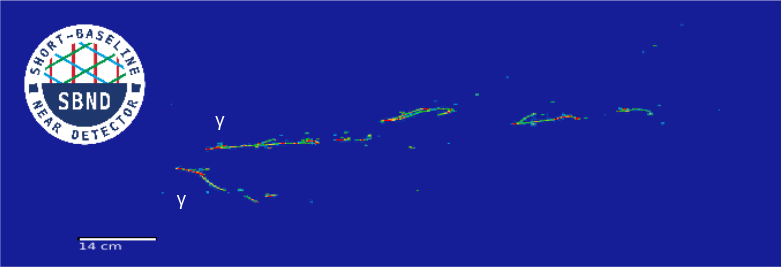
\includegraphics[width=\textwidth]{hnl_2shw}
            \caption{}%
	    \label{fig:hnl_evd_1shw}
        \end{subfigure}
        \centering
        \begin{subfigure}[b]{0.85\textwidth}   
            \centering 
            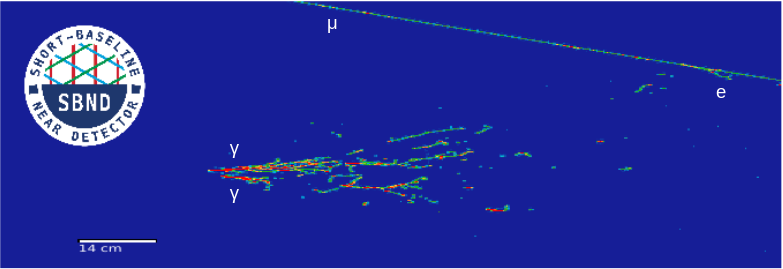
\includegraphics[width=\textwidth]{hnl_1shw}
            \caption{}%
	    \label{fig:hnl_evd_2shw}
	\end{subfigure}
        \caption{
		Event displays showing two different topologies observed from di-photon showers from HNLs. 
	}
        \label{fig:hnl_evd_select}
\end{figure}

%SM neutrino background
Given this signal topology, the first-order background topology from SM neutrino is Neutral Current interactions that produce $\pi^0$ (NC $\pi^0$).
This interaction type also produces di-photon showers without any hadronic activities at vertex.
The second-order background topology is from Charged Current electron (anti-)neutrinos (CC $\nu_e$) interactions.
This interaction type typically produces one or multiple hadrons in addition to a single shower.
However, in some scenarios, the hadrons are too low in energy to be reconstructed, resulting in a single shower topology after reconstruction.
Fig. \ref{fig:ncpi0_evd} shows an event display of the observable di-photon showers from NC $\pi^0$ interaction, which is indistinguishable from the di-photon showers from HNLs.
The key distinction separating HNL showers from these SM neutrino showers is the boosted topology of HNL showers, which is exploited for selection to be detailed in Sec. \ref{sec:hnl_shower_select}.

\begin{figure}[htbp!]
	\centering
        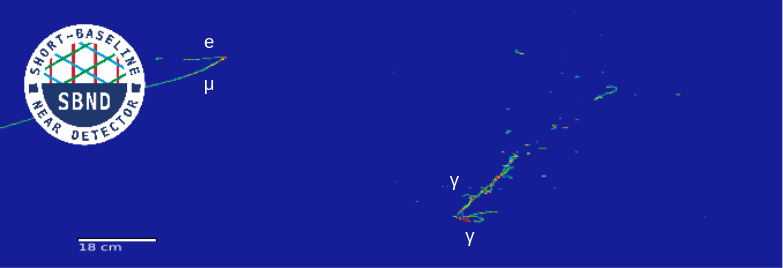
\includegraphics[width=0.85\textwidth]{ncpi0}
        \caption{
		Event display showing di-photon showers from NC $\pi^0$ interactions. 
	}
	\label{fig:ncpi0_evd}
\end{figure}

Moreover, SM neutrino interactions can occur outside the FV, but their products can have sufficient energy to propagate inside the FV.
For those interactions occurring outside the FV but inside the detector, they are considered Non-FV interactions.
For those interactions occurring completely outside of the detector, they are considered dirt neutrinos interactions.
As previously discussed in Sec. \ref{sec:gen_genie}, despite interacting outside of the FV, these interactions can introduce non-negligible backgrounds, especially if their daughter particles produce shower topologies. 

%Cosmic background and CCnumu
Finally, any background interactions that produce tracks are considered as low priority backgrounds since a track topology is easily distinguishable from a shower topology.
From SM neutrinos, these interactions are from Charged Current muon (anti-)neutrinos (CC $\nu_\mu$) or any Neutral Current interactions that do not produce a neutral pion (Other NC).
Track signature for protons is short stubs, whilst track signature for muons and pions, are long tracks.
Fig. \ref{fig:numu_cos_evd} shows an event display of a common observable from CC $\nu_\mu$ interactions that result into a final state of 1 muon and 1 proton.
Similarly, cosmic muons typically leave very long tracks crossing the entire detector with some iconic features such as delta-rays or Michel electrons, which are electrons from muons decay at rest.
Fig. \ref{fig:hnl_evd_2shw} (top right) and Fig. \ref{fig:numu_cos_evd} (bottom left) both show a long cosmic track with some delta-rays along the track.
Meanwhile, Fig. \ref{fig:ncpi0_evd} shows a cosmic muon comes to a stop and eventually decays into a Michel electron.

\begin{figure}[htbp!]
	\centering
        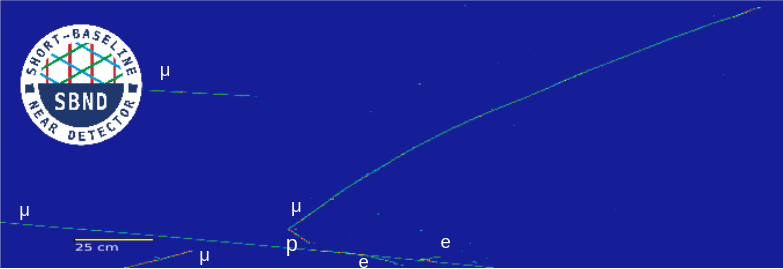
\includegraphics[width=0.85\textwidth]{1m1p_cos}
        \caption{
		Event display showing 1 muon and 1 proton track from CC $\nu_\mu$ interactions. 
	}
	\label{fig:numu_cos_evd}
\end{figure}


%********************************** %First Section  **************************************

\section{Description of MC Samples}

The selection presented in this chapter was performed on Monte Carlo (MC) samples, that were generated using the simulation framework described in Chapter \ref{ChapterSim}.
These samples were then reconstructed using the framework described in Chapter \ref{ChapterReco}.
The following section provides the description for signal and background samples.

For signal samples, HNL signals were overlay with cosmic muons occuring within the TPC readout window. 
In total, 7 samples were generated, where each sample of 60,000 signals corresponds to a mass point ranging between 140 to 260 MeV in step of 20 MeV.
The signals can be re-weighted from the nominal mixing angle $|U_{\mu4}|^{2}$ to another mixing angle $|U'_{\mu4}|^{2}$ by applying a weight as follows
\begin{equation}
    w = \left(\frac{|U_{\mu4}|^{2}}{|U'_{\mu4}|^{2}}\right)^{2}
\end{equation}

For SM neutrino background samples, three samples were produced.
The first one is a core sample entailing all SM neutrino interactions occurring inside the detector volume as well as outside the detector in the \textit{Rockbox} volume, as discussed in Sec. \ref{sec:gen_genie}.
Two additional dedicated samples of enriched NC $\pi^0$ and CC $\nu_e$ backgrounds were also generated, to improve the limited statistics of these interactions in the core sample.
The three samples were normalised to the exposure of $1 \times 10^{21}$ Protons On Target (POT) to account for 3 years on data taking.
This yield approximately $\sim331,000$ NC $\pi^0$ interactions and $\sim33,000$ CC $\nu_e$ interactions which the primary background.
Other background from CC $\nu_\mu$ and other NC interactions make a total of approximately $\sim5$ million interactions.
Meanwhile, an additional $\sim2$ million and $\sim3$ million interactions from Non-FV and dirt interactions are considered as backgrounds, although only a fraction of the might deposit energy in the detector.

Finally, a cosmic-only sample was generated to account for in-time cosmics, as discussed in Sec. \ref{sec:gen_corsika}.
This sample consists of events triggered by a cosmic-only interactions.
However, it is important to note that dedicated trigger efficiency study will be carried out to better understand the rate of in-time cosmic events once SBND is operational.
The cosmic-only sample was also normalised to the target POT, and combined with SM neutrino samples to form a single sample describing the background to the HNL signal.  

The unit of the selection relies on \textit{events}, defined by the triggering of the detector where a single event corresponds to a single trigger.
After reconstruction, each event contains \textit{slices}, a reconstruction unit created by Pandora that encapsulates all energy in the TPC from a single origin, as discussed in Sec. \ref{sec:reco_tpc}.
The equivalent reconstruction unit to a slice from the PDS reconstruction is a \textit{flash}, as discussed in Sec. \ref{sec:reco_others}.
A slice consists of a hierarchy of particles, where each can resemblance a track or a shower.
The selection presented in the forthcoming sections are performed on slices, where slices are accepted or rejected based on the series of cuts using the reconstructed information within the slice or by matching a slice to a flash.

%********************************** %First Section  **************************************

\section{Selection Motivation}

The selection workflow was developed by exploiting distinct features of HNLs, separating signal topologies from background topologies.
One previously stated feature is the boosted topology of HNL showers as depicted in Fig. \ref{fig:hnl_evd_1shw}.
Another feature is the late arrival of HNLs relative to SM neutrinos, as previously depicted in Fig. \ref{fig:beam_modulus} showing the timing distribution of the beam bucket for HNLs and SM neutrinos.
The distribution of SM neutrinos resemblance a Gaussian-shaped bucket as they travel nearly as the speed of light, whilst HNLs travel at a slower velocity and smear the Gaussian.
This is the key distribution for setting the upper limits on the mixing angle $|U_{\mu4}|^2$ of HNLs since it demonstrates the distinct shape difference between the signal and the background.
Thus, the signal-to-noise ratio varies bin-by-bin, where signal-rich bins locate at the edge of the beam bucket (or the Gaussian tails) and background-rich bins locate at the centre of the beam bucket (or the Gaussian peak).
The setting limits procedure, to be detailed in upcoming Chapter \ref{}, employs a multi-binned analysis such that the resulting sensitivity limits depends on the signal-to-noise ratio per bin.
This implies that signal-rich bins are the main factor driving the limits.
With this in mind, the following selection procedure was optimised to achieve a high signal-to-noise ratio with bins located at the edge of the beam bucket distribution.

%********************************** %First Section  **************************************

\section{Cosmic Background Removal}

\subsection{Pandora Unambiguous Cosmic Removal}

Being a surface detector, SBND is exposed to a high rate of cosmic rays, expecting $\sim 185$ million reconstructed slices from cosmics for the target POT of $1 \times 10^{21}$.
As a comparison, the expected rate of reconstructed slices from SM neutrino interactions is $\sim 11$ million slices.
The first step of the selection is cosmic rejection, targeting primarily at removing out-of-time cosmic muons.
Pandora performs an unambiguous cosmic removal early in the reconstruction chain, by reconstructing a slice as a neutrino only if the slice is identified as a non-clear cosmic, as previously described in Sec. \ref{sec:reco_tpc}. 
The selection thus begins with selecting only slices reconstructed as a neutrino as determined by Pandora.
This rejects $90 \%$ of the $\sim 185$ million slices from cosmics, leaving behind only $19.5$ million slices.
Meanwhile, only $0.6 \%$ of the reconstructed slices from HNL signals is removed, with similar reductions across other reconstructed slices from SM neutrino backgrounds.  
As previously stated, the remaining slices after this cut are reconstructed as neutrinos, and consist of a reconstructed vertex and dedicated reconstruction algorithms required by the upcoming cuts.

\subsection{Beam Spill Cut}

The second cut to remove cosmics is to consider the start time of the interaction $\t_0$, by examining the \textit{flash time}, detailed in Sec. \ref{}, matched to a slice, detailed in Sec. \ref{}.  

Only slices matched to a flash are selected, using the flash matching Opt0Finder module detailed in Sec. \ref{reco2:Opt0Finder}.
The time of the matched flash must be within the beam spill window.
In MC, the beam spill window is [0.367, 1.967] $\mu$s, with $t = 0\ \mu$s when the first POT begins.
To account for smearing due to the $z$-length of the detector and PDS reconstruction, the selection window for beam spill is widened to [0.351, 1.983] $\mu$s.
This cut is illustrated in Fig. \ref{fig:cosmic_cut_beamspill}.

\subsection{CRUMBS BDT Cut}

\subsection{Non-Fiducial Volume Cut}

%********************************** %First Section  **************************************
\section{SM Neutrinos Background Removal}

\subsection{Track Removal}

\subsection{Electron Shower Removal}

%********************************** %First Section  **************************************

\section{HNL Shower Selection}
\label{sec:hnl_shower_select}

%********************************** %First Section  **************************************
\subsection{Track-Shower BDT Cut}

\subsection{Calorimetry Cut}

\subsection{Shower Angle Cut}

\subsection{Invariant Mass Cut}

\subsection{Timing Cut}

%********************************** %First Section  **************************************

\section{Final Selection Results}

%********************************** %First Section  **************************************

\section{Truth Study On Timing Resolution Improvement}

%********************************** %First Section  **************************************

\section{Concluding Remarks}

